\section{System Architecture}
\label{sec:architecture}

HybridCloudSim is a discrete event simulator built on SimPy. It models a hybrid cloud at the \emph{orchestration} layer: job arrival, device selection, capacity blocking, iterative quantum classical execution, and the resulting energy and cost. Circuit level quantum behavior is deliberately abstracted; device service times are obtained from analytical performance models parameterized by published hardware specifications, so that a full run over thousands of jobs completes in seconds on a single core.

\subsection{Overview}
\label{sec:arch-overview}

\begin{figure}[t]
\centering
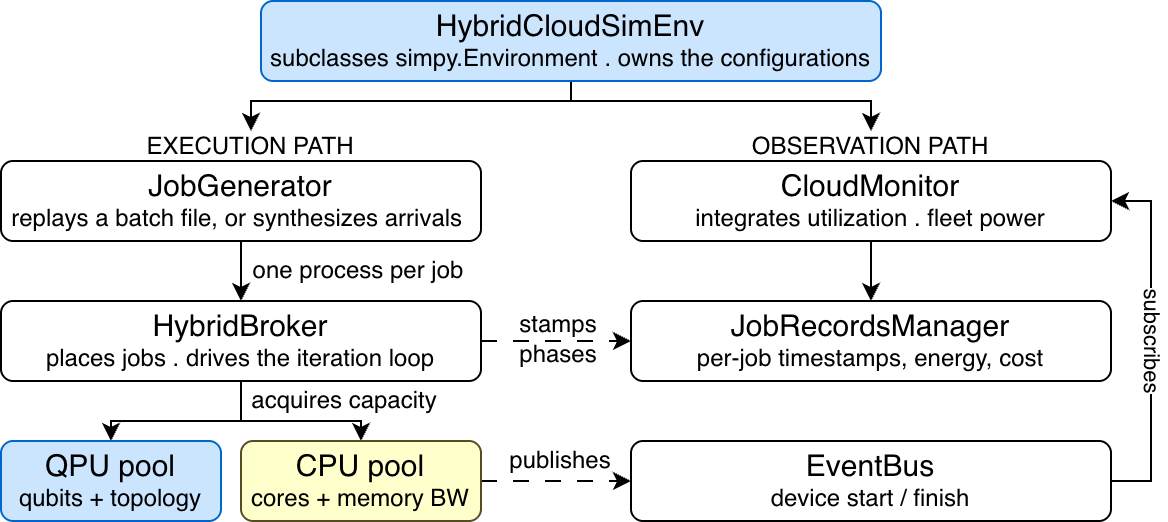
\includegraphics[width=0.99\linewidth]{Images/architecture.png}
\caption{Component structure of HybridCloudSim. Both paths descend from the composition root, but they never join: the execution path (left) places jobs and consumes device capacity, while the observation path (right) only records what the execution path has already committed. Dashed links carry telemetry and never influence placement.}
\label{fig:architecture}
\end{figure}

The simulation framework is organized around a single composition root, \texttt{HybridCloudSimEnv}, which subclasses the SimPy environment and instantiates every other component. Table~\ref{tab:components} summarizes the roles. Control flows top down, where the job feed creates one broker process per job, and each broker drives devices. Observability flows bottom up: devices emit events on a publish subscribe bus and write per job records that the monitor and the records manager aggregate.

\begin{table}[t]
\centering
\caption{Principal components of HybridCloudSim.}
\label{tab:components}
\small
\begin{tabular}{@{}ll@{}}
\toprule
\textbf{Component} & \textbf{Responsibility} \\
\midrule
\texttt{HybridCloudSimEnv} & Composition root; owns the cost model \\
\texttt{JobGenerator}      & Trace replay or stochastic arrivals \\
\texttt{HybridBroker}      & Per job scheduling and phase control \\
\texttt{QuantumDevice}     & Qubit capacity, topology, QPU time \\
\texttt{CPU}               & Core and memory bandwidth capacity \\
\texttt{EventBus}          & Decoupled device event notification \\
\texttt{CloudMonitor}      & Utilization integration, fleet power \\
\texttt{JobRecordsManager} & Event log, and job metrics \\
\bottomrule
\end{tabular}
\end{table}

A run is fully specified by three inputs: a device inventory (a list of QPU and CPU objects), a workload (a trace file or an arrival process), and a cost configuration. Devices are constructed detached from the environment and are bound to it in a separate initialization pass, at which point their SimPy containers and resources are created. This two phase construction keeps device definitions declarative and makes parameter sweeps explicit: because devices carry mutable state, specifically qubit containers, the topology graph, and the qubit occupancy map, a fresh inventory is instantiated for each configuration in a sweep. 

Figure~\ref{fig:architecture} makes this separation explicit. The execution and observation paths descend from the same root but never join: the broker consults device capacity in order to place work, whereas the event bus, the cloud monitor, and the records manager only ever read state that the execution path has already committed. No scheduling decision depends on a telemetry value. This asymmetry is what allows instrumentation to be as dense as the analysis requires; every phase transition of every job is stamped, and every device transition is published, without perturbing the schedule under study. It also fixes the provenance of each reported quantity: phase boundaries originate in the broker, device arrivals in the devices themselves, time integrated utilization and instantaneous fleet power in the monitor, and per job energy and cost in the records manager. We rely on that provenance in Section~\ref{sec:arch-telemetry}, where the two independently computed energy figures are reconciled.

\subsection{Workload}
\label{sec:arch-workload}

A job is a tuple
$J=(n, d, s, p, a, r, c, b)$
giving qubit count $n$, circuit depth $d$, shot count $s$, priority $p$, arrival time $a$, required iterations $r$, CPU units $c$, and memory bandwidth $b$. Jobs enter the system in one of two modes. In \emph{dispatcher} mode the generator replays a CSV or JSON trace, releasing each job at its recorded arrival time; this is the mode used for all experiments in this paper, since it makes workloads reproducible and shareable. In \emph{generator} mode jobs are synthesized online from a configurable inter arrival distribution (exponential by default) with randomized circuit parameters. In both modes the generator spawns one broker process per job, so concurrency in the model is bounded by device capacity rather than by any fixed pool of workers.

\subsection{Broker and Execution Lifecycle}
\label{sec:arch-broker}

The broker is the scheduling core. Each job executes $r$ variational iterations, and every iteration consists of a QPU phase followed by a CPU phase, reflecting the structure of VQE and QAOA style workloads in which measurement outcomes are returned to a classical optimizer that produces the next parameter set. Algorithm~\ref{alg:broker} states the loop.

\begin{algorithm}[t]
\caption{Broker process for job $J$}
\label{alg:broker}
\begin{algorithmic}[1]
\State $i \gets 0$
\While{$i < r$}
  \State $q \gets \Call{Select}{\mathrm{QPU}, n}$
  \While{$q = \mathrm{null}$} \Comment{no device has free capacity}
    \State \textbf{wait} $\delta$;\quad $q \gets \Call{Select}{\mathrm{QPU}, n}$
  \EndWhile
  \State \Call{Execute}{$q$, $J$};\quad \Call{Record}{$J$, QPU}
  \State $u \gets \Call{Select}{\mathrm{CPU}, (c,b)}$
  \While{$u = \mathrm{null}$}
    \State \textbf{wait} $\delta$;\quad $u \gets \Call{Select}{\mathrm{CPU}, (c,b)}$
  \EndWhile
  \State \Call{Execute}{$u$, $J$};\quad \Call{Record}{$J$, CPU}
  \State $i \gets i + 1$
\EndWhile
\State \Call{FinalizeEnergyAndCost}{$J$}
\end{algorithmic}
\end{algorithm}

\textsc{Select} filters the inventory to devices of the requested type that are not under maintenance and whose free capacity meets the request, namely free qubits for a QPU, free cores \emph{and} free memory bandwidth for a CPU, and returns the most lightly loaded candidate, breaking ties in favor of the device with the largest residual capacity. When no candidate exists the broker retries after a fixed polling interval $\delta$ rather than enqueueing, which keeps the admission decision re-evaluated against current fleet state. The resulting blocking behavior, rather than an explicit queue discipline, is what produces the contention observed in Section~\ref{sec:use-cases}. The policy is localized in \textsc{Select}, so alternative disciplines (priority, fair share, energy aware placement) can be substituted without touching the phase loop.
